\documentclass[border=4pt]{standalone}
% Preámbulo común de las figuras. Cada figura es un documento standalone
% que se compila a SVG con scripts/build_figures.sh
\usepackage[utf8]{inputenc}
\usepackage{amsmath}
\usepackage{tikz}
\usepackage[american, siunitx]{circuitikz}
\usetikzlibrary{arrows.meta,calc,decorations.pathmorphing,patterns}
\tikzset{
  >={Stealth[length=2.2mm]},
  eje/.style={->, thin},
  hilo/.style={thick},
}
% Paleta común: tonos medios legibles sobre fondo claro
\definecolor{azul}{RGB}{31,94,168}
\definecolor{rojo}{RGB}{192,57,43}
\definecolor{verde}{RGB}{39,128,73}
\definecolor{naranja}{RGB}{211,120,30}
\definecolor{morado}{RGB}{125,60,152}

\begin{document}
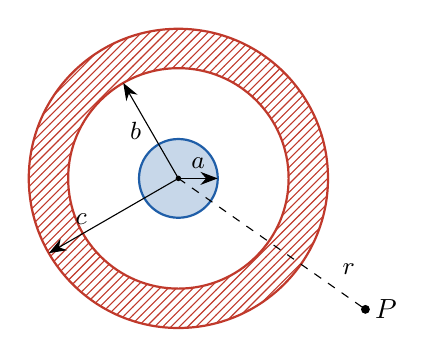
\begin{tikzpicture}[scale=1.0]
  \fill[pattern=north east lines, pattern color=rojo] (0,0) circle (1.9);
  \fill[white] (0,0) circle (1.4);
  \draw[rojo, thick] (0,0) circle (1.9);
  \draw[rojo, thick] (0,0) circle (1.4);
  \filldraw[draw=azul, fill=azul!25, thick] (0,0) circle (0.5);
  \fill (0,0) circle (1pt);
  \draw[->] (0,0) -- (0.5,0) node[midway, above, font=\small]{$a$};
  \draw[->] (0,0) -- (120:1.4) node[midway, left, font=\small]{$b$};
  \draw[->] (0,0) -- (210:1.9) node[pos=0.75, above, font=\small]{$c$};
  \draw[dashed] (0,0) -- (-35:2.9);
  \fill (-35:2.9) circle (1.6pt) node[right]{$P$};
  \node[font=\small] at (-28:2.45) {$r$};
\end{tikzpicture}
\end{document}
